% Two escape criteria: leaving Dimorphos is not leaving the binary.
% Compile from `docs/preprint`:  lualatex sekil/kacis.tex
\documentclass[border=3pt,tikz]{standalone}
\usepackage{amsmath}
\usepackage[outline]{contour}
\usetikzlibrary{calc,arrows.meta,decorations.markings,patterns}
\contourlength{1.0pt}
\tikzset{>=latex}

\colorlet{ink}{black!82}
\colorlet{gh}{black!42}
\colorlet{backcol}{red!72!black}      % falls back
\colorlet{boundcol}{orange!88!black}  % bound to the binary
\colorlet{freecol}{blue!55!cyan!75!black} % leaves the system

\begin{document}
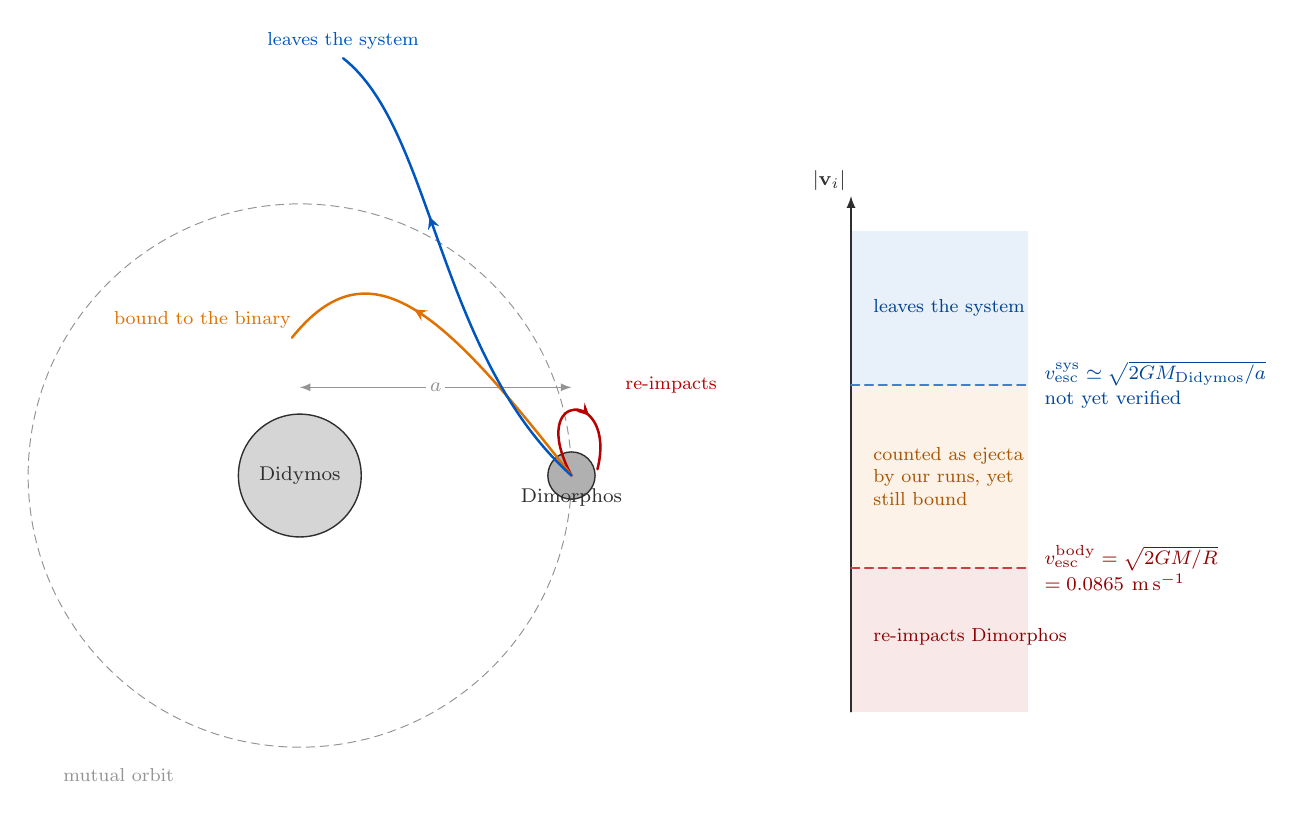
\begin{tikzpicture}[
    font=\footnotesize, line cap=round,
    thin_/.style={line width=0.35pt, draw=gh},
    traj/.style={line width=0.9pt, draw=#1,
      postaction={decorate, decoration={markings,
        mark=at position 0.62 with {\arrow[draw=#1]{stealth}}}}},
  ]

% ===================== (a) the binary ==================================
\coordinate (K) at (0,0);
\coordinate (D) at (3.45,0);

\draw[thin_, densely dashed] (K) circle (3.45);
\node[gh, scale=0.85, anchor=north] at (-2.3,-3.62) {mutual orbit};

\fill[ink!20, draw=ink, line width=0.5pt] (K) circle (0.78);
\node[ink, scale=0.9] at (K) {Didymos};

\fill[ink!38, draw=ink, line width=0.5pt] (D) circle (0.30);
\node[ink, scale=0.9, anchor=north, inner sep=5pt] at (D) {Dimorphos};

\draw[thin_, <->] ($(K)+(0,1.12)$) -- ($(D)+(0,1.12)$)
   node[midway, fill=white, inner sep=1.5pt, text=gh, scale=0.9] {$a$};

% --- three fates -------------------------------------------------------
% 1. below the body's own escape speed: falls back
\draw[traj=backcol] (D) .. controls ($(D)+(118:1.25)$) and ($(D)+(62:1.25)$)
   .. ($(D)+(0.33,0.08)$);
% 2. above it, below the system's: leaves Dimorphos, stays bound
\draw[traj=boundcol] (D) .. controls ($(D)+(128:2.6)$) and (0.9,3.0)
   .. (-0.1,1.75);
% 3. above both: leaves the system
\draw[traj=freecol] (D) .. controls ($(D)+(138:2.3)$) and (1.7,4.4)
   .. (0.55,5.3);

\node[backcol, scale=0.85, anchor=west, inner sep=2pt] at ($(D)+(0.62,1.15)$)
   {\contour{white}{re-impacts}};
\node[boundcol, scale=0.85, anchor=south east, inner sep=2pt] at (-0.05,1.8)
   {\contour{white}{bound to the binary}};
\node[freecol, scale=0.85, anchor=south, inner sep=2pt] at (0.55,5.35)
   {leaves the system};

% ===================== (b) the speed ladder ============================
\begin{scope}[shift={(7.0,-3.0)}]
  \def\H{6.1}
  \pgfmathsetmacro{\yA}{0.30*\H}   % v_esc of the body
  \pgfmathsetmacro{\yB}{0.68*\H}   % v_esc of the system

  \fill[backcol!9]  (0,0)    rectangle (2.25,\yA);
  \fill[boundcol!9] (0,\yA)  rectangle (2.25,\yB);
  \fill[freecol!9]  (0,\yB)  rectangle (2.25,\H);

  \draw[->, ink, line width=0.5pt] (0,0) -- (0,\H+0.45)
     node[anchor=south east, scale=0.9, inner sep=2pt]
     {$|\mathbf v_i|$};

  \draw[backcol!75, line width=0.7pt, densely dashed] (0,\yA) -- (2.25,\yA);
  \draw[freecol!75, line width=0.7pt, densely dashed] (0,\yB) -- (2.25,\yB);

  \node[anchor=west, scale=0.88, text=backcol!80!black, align=left]
    at (2.35,\yA)
    {$v_{\rm esc}^{\rm body}=\sqrt{2GM/R}$\\[1pt]
     \textbf{$=0.0865\ \mathrm{m\,s^{-1}}$}};
  \node[anchor=west, scale=0.88, text=freecol!80!black, align=left]
    at (2.35,\yB)
    {$v_{\rm esc}^{\rm sys}\simeq\sqrt{2GM_{\rm Didymos}/a}$\\[1pt]
     not yet verified};

  \node[anchor=west, scale=0.85, text=backcol!75!black] at (0.18,{0.52*\yA})
    {re-impacts Dimorphos};
  \node[anchor=west, scale=0.85, text=boundcol!75!black, align=left]
    at (0.18,{0.5*(\yA+\yB)})
    {counted as ejecta\\by our runs, yet\\still bound};
  \node[anchor=west, scale=0.85, text=freecol!75!black] at (0.18,{0.5*(\yB+\H)})
    {leaves the system};
\end{scope}

\end{tikzpicture}
\end{document}
